\documentclass[journal]{IEEEtran}

\usepackage{lineno,hyperref}
\usepackage{amsmath}
\usepackage{graphicx}
\usepackage{caption}
\usepackage{subcaption}
\usepackage{titlesec}
\usepackage[normalem]{ulem}
\usepackage[dvipsnames]{xcolor}
% \definecolor{mygray}{gray}{0.6}

\newcommand{\note}[1]{\textcolor{gray}{#1}}
\newcommand{\todo}[1]{\textcolor{blue}{TODO: }\textcolor{gray}{ #1}}

\begin{document}
\title{A paper}
\date{\vspace{-5ex}}
\author{Someone}
\maketitle

\section{Introduction}



\begin{figure}[h!]
    \centering
    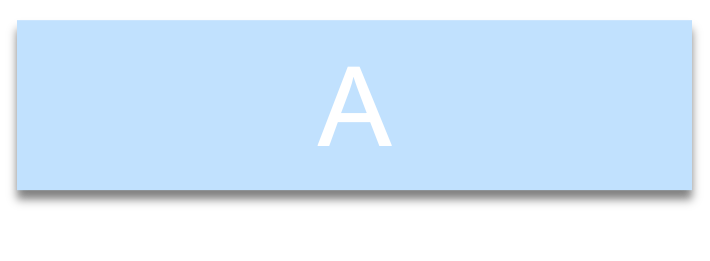
\includegraphics[height=4cm]{media/a_picture.png}
    \caption{A picture.}
    \label{fig:picture}
\end{figure}

Consider the problem \cite{paper}.


\bibliographystyle{IEEEtran}
\bibliography{refs/refs}


\end{document}